% file: tree-with-names.tex

\documentclass{standalone}
\usepackage{tikz}
\usepackage{tikz-qtree}

\begin{document}
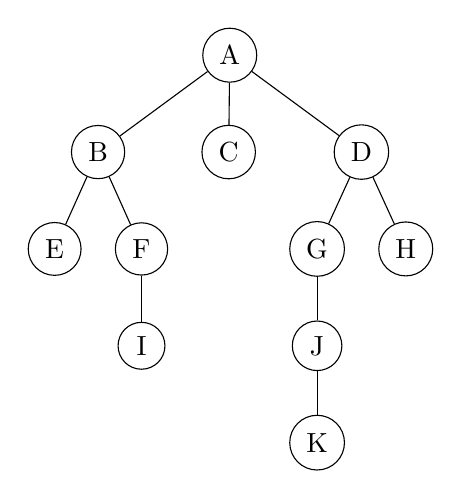
\begin{tikzpicture}[level distance = 35pt, sibling distance = 12pt,
  edge from parent/.style= { % added code
      draw, edge from parent path = {(\tikzparentnode) -- (\tikzchildnode)}}]
  \tikzset{every tree node/.style = 
    {align = center, circle, draw}}

    \Tree [.{A}	[.{B} [.{E} ]
		     [.{F} [.{I} ]]
                ]
		[.{C} ]
		[.{D} 
		  [.{G} 
		    [.{J} [.{K} ]] 
		  ] 
		  [.{H} ]
		] 
	  ]
  \end{tikzpicture}
\end{document}
